\vspace{-0.15in}
\section{Numerical Evaluation}
\label{sec:Numerical Evaluation}
%
% \begin{figure}[t!]
% \centering
% 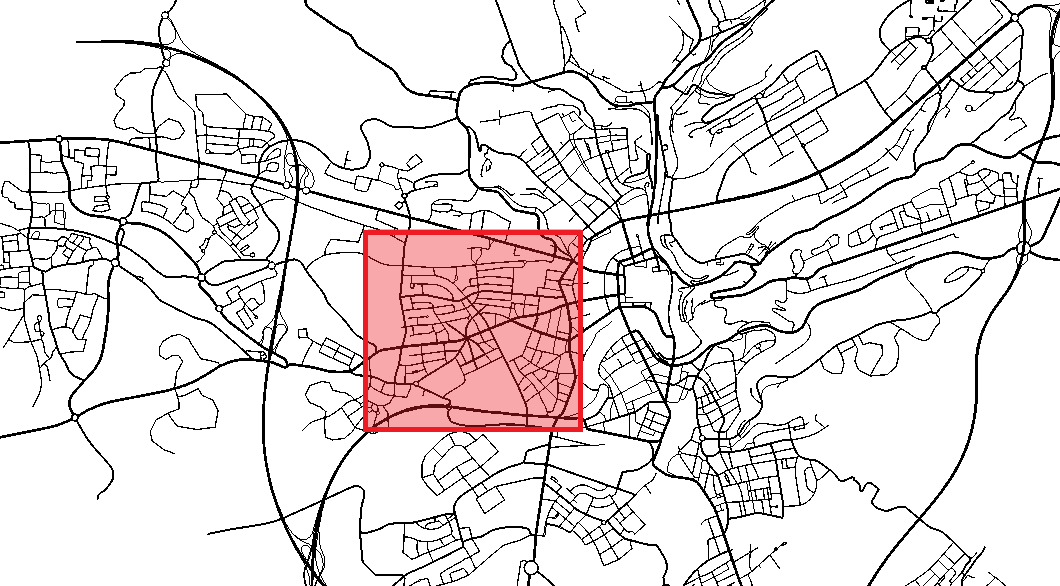
\includegraphics[width=1\columnwidth]{figures/LuxCity.png}
% \caption{Map and road grid of Luxembourg City center. The area within the red square corresponds to the region considered in our simulations.\vspace{-0.2in}}
% \label{fig:luxCity}
% \end{figure}
%
\begin{figure}[t!]
\centering
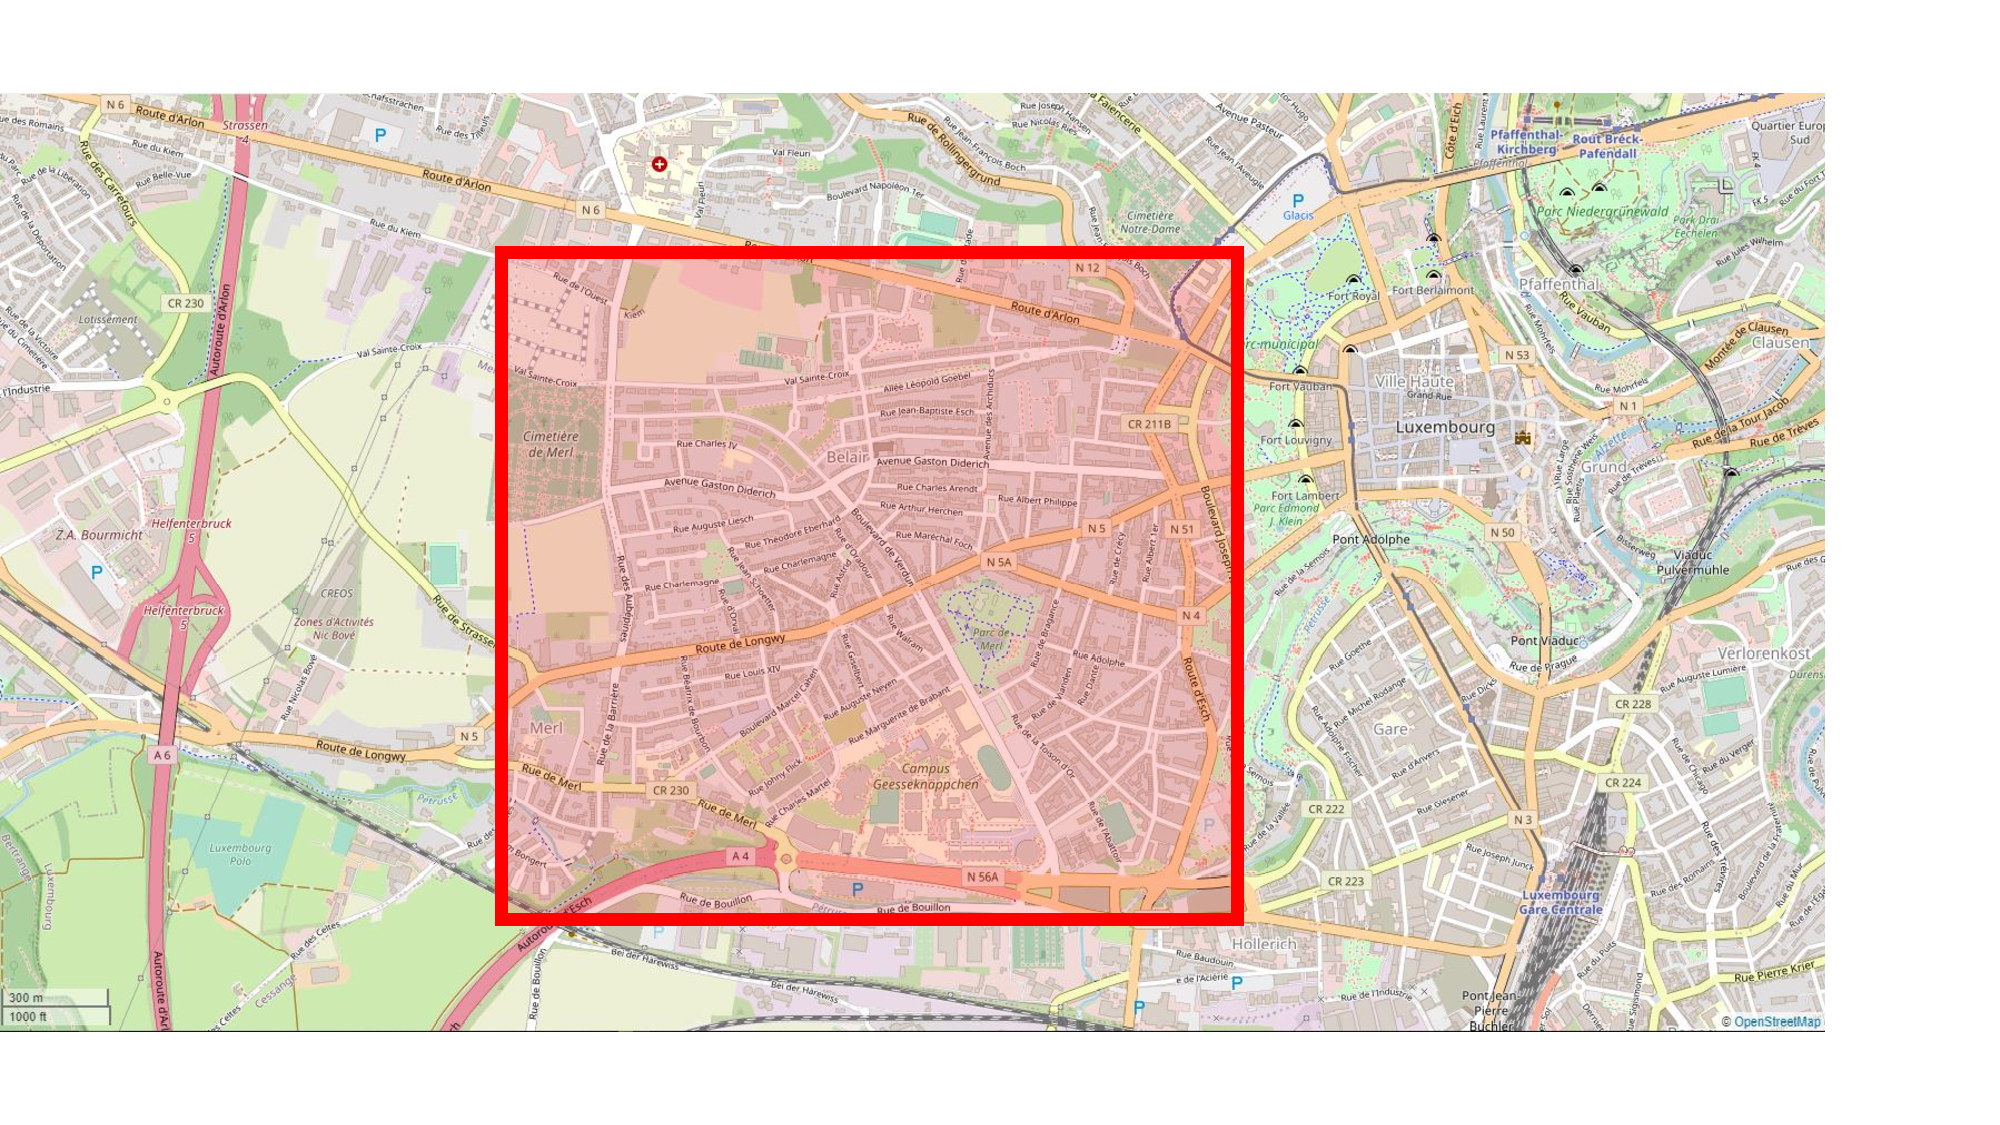
\includegraphics[width=1\columnwidth]{figures/lux_map_2.pdf}
\caption{Map and road grid of Luxembourg City center. The area within the red square corresponds to the region considered in our simulations.\vspace{-0.2in}}
\label{fig:luxCity}
\end{figure}

%
% \begin{figure}[b!]
% \centering
% 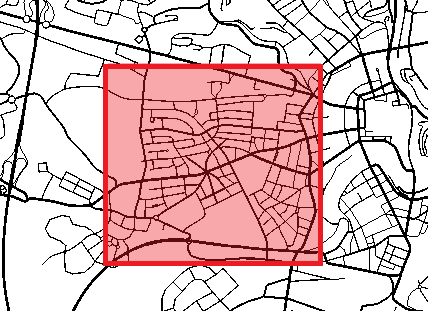
\includegraphics[width=1\columnwidth]{figures/LuxCitySmall.png}
% \caption{City center of the Luxembourg city. \vspace{-0.2in}}
% \label{fig:luxCity}
% \end{figure}

In this section we present the results of the numerical assessment of our framework for decentralized Gossip Learning.
In order to implement a realistic scenario in our simulation experiments, we adopted the dataset of the Luxembourg
SUMO Traffic (LuST) Scenario \cite{lux}, consisting in measurement-based vehicular traces over 24 hours from the city of Luxembourg, with a typical topology common in mid-size European cities, and with realistic traffic demand and mobility patterns. In particular, we considered a square region of side $1050$ m (\fref{fig:luxCity}) in the city center, within which we assumed that predictions of vehicle trajectories are required. We partitioned such region into $49$ square cells of side $150$ m, compatibly with the case in which each cell corresponds to the coverage area of a MEC-enabled small cell base station. As in many real scenarios, vehicular traffic flows exhibit non-stationary properties which might affect the accuracy of our GL trained models. In order to limit such effects of the variations of traffic flows over time, we observed the performance of our scheme over a time interval of one hour (specifically, from $6:30$ AM to $7:30$ AM, where vehicular traffic is sufficiently intense and stationary). Such time interval has been chosen to be, on one side, long enough to allow our training framework to progress substantially, but short enough for the average pattern of vehicular traffic flows not to vary significantly. In the given region, on average about $300$ vehicles are present at every time instant in the time interval considered, and every vehicle is in the range of about $60$ other vehicles, of which on average only half are in the exploitation phase and are thus able to act as clients.\\
%\footnote{\com{here I'd like exact numbers: memo for next time.}}\\
For implementing the simulations of opportunistic communications among vehicles, we adopted the Omnet++~\cite{Varga2010} framework, while Keras~\cite{chollet2018deep} was used for implementing our GL algorithm. We assumed vehicles sample their position in space every $5$ s, i.e. at rate comparable to that common in many present day car fleet management applications. Moreover, we assumed to require a prediction about a vehicle's position in $10$ seconds in the future. Such forecast horizon is of the same order of magnitude of those required in, e.g., predictive collision avoidance systems, or in MEC resource preallocation strategies. Our LSTM model input being composed by $24$ steps, it requires at least the last two minutes of the trajectory of a car in order to issue a trajectory prediction. 
%The goal of this work however is not reaching maximum accuracy or precision on the specific trajectory dataset. Rather, we wish to compare different methods to predict the vehicle trajectory in the next $10$ seconds. 
%We thus choose reasonable values for hyper-parameters, following indications in the literature. 
We considered each node performs model training over its entire local dataset, adopting a local batch size of $32$ data points (coherently with the indications in \cite{bengio2012practical} \cite{masters2018revisiting}, and a $10^{-3}$ learning rate, as suggested in ~\cite{geron2019hands}.\\
Given that in the scenario considered the average sojourn time of vehicles in the given region has been around $20$ minutes, after several experiments for each node we have chosen for the initialization phase a duration of about half of this time, i.e. $9$ m $30$ s. Indeed in the given setting such a duration is, on one side, short enough to have a substantial amount of nodes in the exploitation stage at each point in time (about $50\%$), and thus contributing to our collaborative training. On the other, it is long enough to have a substantial training set at each node, and thus to allow the collaborative training to progress at a reasonable rate within the residual sojourn time of each vehicle. Given the relatively short duration of the exploitation phase, we have experimentally verified that the periodic training of the local model instance on the local database during the exploitation phase has no significant impact on model accuracy. Note however that these considerations are strictly related to the characteristics of the chosen scenario, and specifically, to the size and shape of the given region, as well as the mean node speed. In order to perform a first evaluation of our approach, we have assumed that the tasks of model training, of computing a meta-model, and of exchanging a model are instantaneous, thus modeling the case in which the limiting factor of our training framework is given by the way in which training and meta-model computing task are implemented, rather than by their duration.\\       
% Therefore, each client initializes its weights randomly and trains the received models on the entire dataset. In the following we evaluate our algorithms with a fixed test set and short rolling test set.
% \footnote{\com{there should also be periodically, a training of the local model over its own data. This is important because due to the clean slate assumption, the dataset is small, and data accumultaed after the initialization phase may substantially improve the model. But how often? INCLUDED IT IN THE ALGO, BUT NUMERICALLY SAY THAT WE DID NOT DO IT BECAUSE DATASET WERE SMALL.}}
%%%%%%%%%%%%%%%%%%%%%%%%%%%%%
%In the following, we evaluate the performance of the proposed algorithms (DFed Avg, DFed Pow, and DFed MinLoss) through an online learning method. We update  models at each time interval when new data becomes available. We check the availability of data every five seconds.\\
\begin{figure}[t!]
\centering
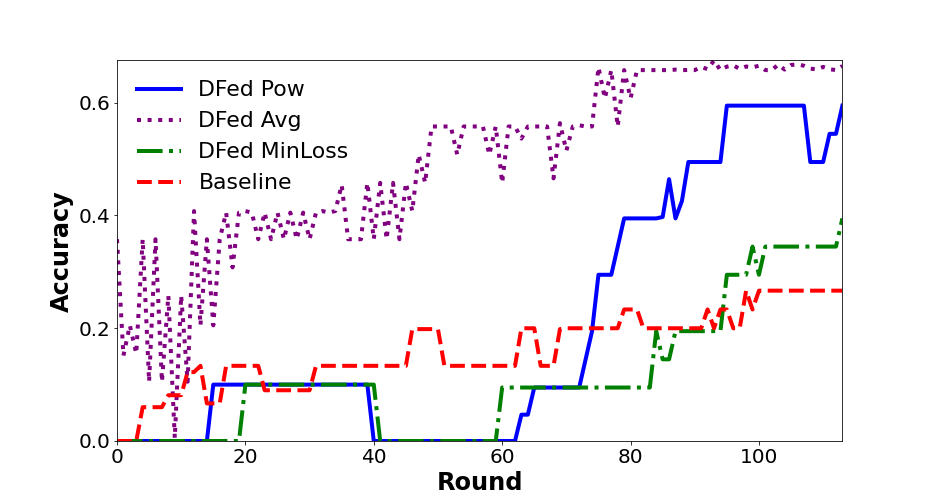
\includegraphics[width=1\columnwidth]{figures/accFixTest3.png} 
\caption{Mean accuracy versus iterations for our GL algorithm, for the three model merging schemes, and baseline model, with static test set, in the Luxembourg scenario.\vspace{-0.3in}}
\label{fig:accuracy}
\end{figure}
%
\begin{figure}[t!]
\centering
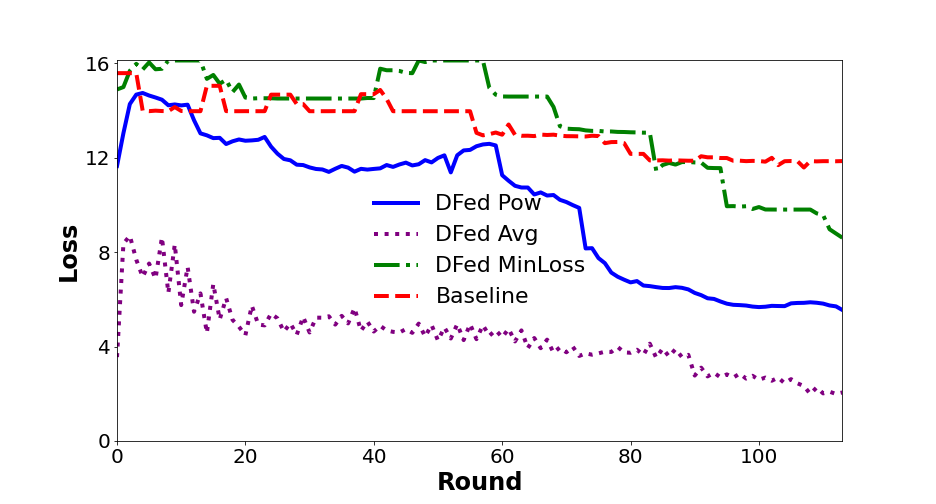
\includegraphics[width=1\columnwidth]{figures/lossFixedSet3.png} 
\caption{Mean loss versus iterations for our GL algorithm, for the three model merging schemes and baseline model with static test set, in the Luxembourg scenario. \vspace{-0.2in}}
\label{fig:loss}
\end{figure}
%
In order to assess the performance of the training process, the test set consisted in the data points of the trajectory of each vehicle within the last $5$ minutes of the vehicle's sojourn time within the given region. With such a choice for the test set (henceforth denoted as \textit{static}), at each point in time during the exploitation stage the evaluation is done on data points about parts of the map which are generally far from those in which the node is located. This holds also, on average, for the dataset of the client nodes. Finally, in order to better appreciate in what measure our collaborative training improves over purely local training, we have considered this latter approach as as a baseline, and we have characterized its performance.\\
\fref{fig:accuracy} and \fref{fig:loss} show accuracy and loss of our GL schemes, averaged over the $30$ cars in the area with longest sojourn time, for the static test set approach. As these figures show, one consequence of choosing a  static test set is that on average the initial loss is high (and the accuracy low) for all of the three meta-model building approaches, and sometimes even lower than the baseline. The figures also show that these parameters keep on improving steadily across the iterations of our GL training scheme.\\
These results show also that despite every node enters the scenario with an empty dataset, a substantial improvement in model accuracy can be achieved within a relatively small amount of rounds. The two plots indicate that, when vehicles spend a sufficiently large amount of time in the scenario, GL schemes can collaboratively train models which achieve a substantially better performance with respect to their initial, locally trained models, and over relatively short timespans.
Moreover, the plots \fref{fig:accuracy} and \fref{fig:loss} seem to suggest that, as expected, the main potential factor contributing to such improvement is the progress in model training, i.e. the gradual inclusion over time in the trained model of an ever larger amount of data about trajectories in the given region.\\ 
%This approach shows the performance of the trained model at the end of the vehicle's sojourn time, after that a sufficient amount of training cycles . In a sense thus, and thus it gives an idea of the best possible prediction performance achievable in such a clean-slate scenario.  
%The main performance metric in classification algorithms is accuracy, defined as the percentage of correctly classified outputs.
As for the relative performance of the three approaches to meta-model elaboration, \fref{fig:accuracy} and \ref{fig:loss} show that weighting each contribution to the meta-model based on the relative size of the local training set, outperforms approaches based on loss estimation. This might be due to the fact that while the validation set (over which loss is evaluated in the \textit{DFed Pow} and \textit{DFed MinLoss} approaches) consists in the last $V$ slots of a user's trajectory, and thus to a region of space very close to where the user will be in $h$ slots, the test set is relative to a portion of the user trajectory which is (generally, except for the final part of the vehicle's trajectory) far enough from the current vehicle position (and from where it will be) to make the performance over the validation set not indicative of the actual prediction accuracy of the model. I.e., as the model evolves constantly to adapt its performance to the specific prediction task and to the context in which the prediction is formulated, it would make more sense to take as test set data points which are as much as possible related to that same spatio-temporal context.\\
In order to address this issue, in a new set of experiments, at each time slot $t$ we have adopted as test set the data points relative to the time interval ${(i-l,i+h)}$ where $l$ is the length of the LSTM input (24 slots), and $h$ is the forecast horizon (equal to 2 slots in our experiments). This should allow a more relevant assessment of model performance, as it is performed over the same segment of a vehicle trajectory over which the prediction is performed. 
% In this experiment, after every communication round we evaluated the generated meta-model on the short size rolling test set. The test set at time interval $i$ is constituted of those samples associated to the time interval ${(i-l,i+h)}$ where $l$ is the time duration of the input sequence, and $h$ is the forecast horizon. In our case, $l$ corresponds to a total of 120 seconds of past samples, and $h$ corresponds to the next ten seconds from the current moment.\\
%
\begin{figure}[t!]
\centering
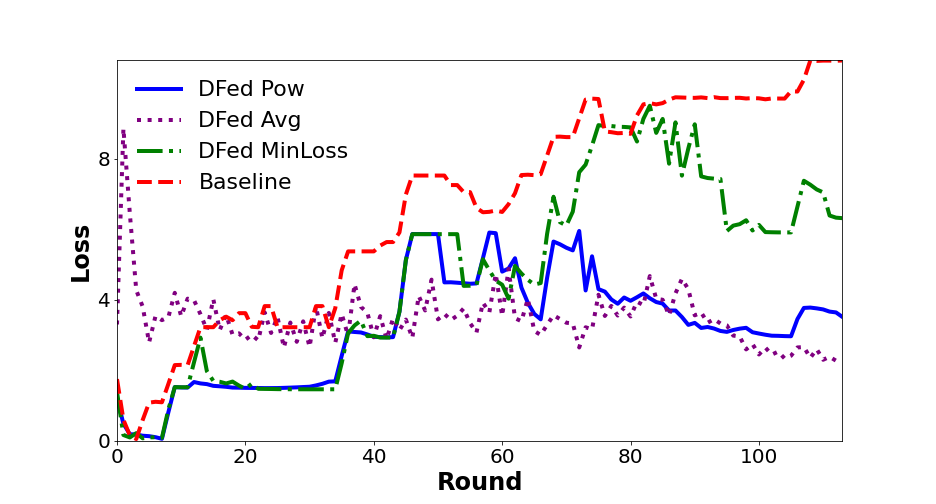
\includegraphics[width=1\columnwidth]{figures/lossShortRolling3.png} 
\caption{Mean loss versus iterations for our GL algorithm with a short size rolling test set, for the three model merging schemes, in the Luxembourg scenario. \vspace{-0.2in}}
\label{fig:lossS}
\end{figure}
%
\begin{figure}[t!]
\centering
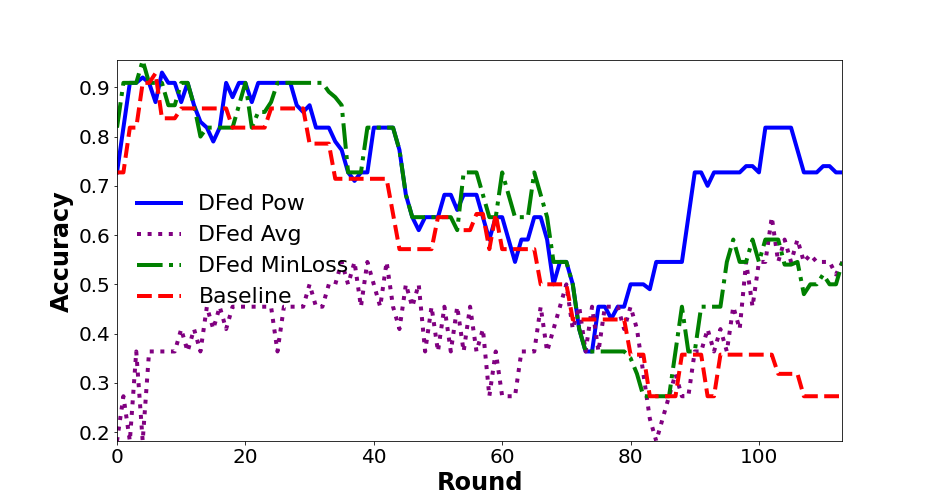
\includegraphics[width=1\columnwidth]{figures/accShortRoll3.png} 
\caption{Mean accuracy versus iterations for our GL algorithm with a short size rolling test set, for the three model merging schemes, in the Luxembourg scenario.\vspace{-0.3in}}
\label{fig:accuracyS}
\end{figure}
As \fref{fig:lossS} and \ref{fig:accuracyS} show, when assessed with a rolling test set the performance (both in terms of accuracy and of loss) of the models trained with our GL approach is generally less pessimistic than with a static test set. In addition, it remains approximately constant as the number of rounds increases, if not for fluctuations which are due to spatial in homogeneities in node density, in the structure of the road grid, and to bursts of nodes arriving and leaving the considered region. Moreover, in this setting the loss-based meta model building approaches perform generally better than the strategy based on the relative size of the local dataset of client nodes, with the DFed Pow performing slightly better than the DFed MinLoss. This is likely due to the fact that test set and validation set are now relative to contiguous regions of space and time interval, making loss measured over the validation set a more relevant indicator of the performance over the (rolling) test set. Note that improvement over the baseline becomes noticeable only after that a substantial amount of rounds has passed. This is due to the fact that the baseline algorithm has been obtained via training over a dataset which typically contains only a very limited number of cell transitions. Thus, it performs poorly whenever the node moves to another cell, an event whose likelihood grows with time, thus steadily worsening the performance of the purely locally trained model over time.  
% DFed Pow and DFed MinLoss show very similar behaviours in the first 70 rounds.
% DFed Avg from communication round 34 to 76 shows an almost constant performance, while DFed Pow and DFed MinLoss exhibit a performance deterioration.
% By looking in detail at datasets, we could see that in this time interval many nodes are moving to a new cell, and this makes the two algorithms worsen their performance in predicting the future trajectory. 
%are two. On one side, such improvement might reflect
%, i.e. as  nodes get closer to that part of the given region in which the test set data points are located. 
%These experiments show thus that the locality of the data on which models are trained plays a key role in improving the trained model over GL. That is, models trained through our GL scheme show significant improvements when the training set used for training (by the node itself, or by clients nodes in the GL scheme) belongs to the vicinity of the area by which the predicting node will pass in the near future.\\
%{\color{red}WE NEED TO SAY SOMETHING MORE ABOUT COMPARISONS.}
